% 原始材料：上级目录「成都七中2029届高一上学期半期考试数学卷」图片 1–4（试题）、5–9（答案）。
\documentclass[UTF8,a4paper,12pt]{ctexart}
\usepackage[margin=2cm]{geometry}
\usepackage{amsmath,amssymb,needspace,fancyhdr,tikz}
\pagestyle{fancy}\fancyhf{}\fancyfoot[C]{\thepage}\renewcommand{\headrulewidth}{0pt}
\setlength{\parindent}{0pt}\setlength{\parskip}{4pt}
\newcommand{\subq}[1]{\par（#1）}
\newcommand{\q}[1]{\par\textbf{#1．}}
\newcommand{\opts}[4]{\par\noindent\makebox[.25\linewidth][l]{A．#1}\makebox[.25\linewidth][l]{B．#2}\makebox[.25\linewidth][l]{C．#3}D．#4}
\newcommand{\pick}{（\hspace{1em}）}
\newcommand{\blank}{\underline{\hspace{3cm}}}
\begin{document}
\begin{center}{\LARGE 成都七中2029届高一半期考试数学试卷}\\[5pt]2026—2027学年度上期\qquad 时间：120分钟\qquad 满分：150分\end{center}
姓名：\blank\qquad 班级：\blank

\textbf{一、单项选择题}（共8小题，每小题5分，共40分。每小题只有一项符合题目要求。）
\q{1}设全集 $U=\{x\mid x\text{是小于9的正整数}\}$，集合 $A=\{1,3,5,7,8\}$，则 $\complement_U A=$\pick
\opts{$\{2,4\}$}{$\{2,6\}$}{$\{2,4,6\}$}{$\{1,2,4,6\}$}
\q{2}已知 $a>b>0$，则下列说法正确的是\pick
\opts{$a^2>b^2$}{$ac^2>bc^2$}{$2^a<2^b$}{$\frac1a>\frac1b$}
\q{3}函数 $f(x)=\sqrt{-3x^2+18x-27}$ 的定义域为\pick
\opts{$\mathbb R$}{$\{3\}$}{$(-\infty,3)\cup(3,+\infty)$}{$[3,+\infty)$}
\q{4}一种产品原来的年产量是1000件，今后 $m$ 年内，计划使产量平均每年比上一年增加 $8\%$，则年产量 $y$（单位：件）关于经过的年数 $x$ 的函数解析式为\pick
\par A．$y=1000(1+8\%\cdot x)$\hfill B．$y=1000(1+8\%)^{mx}$\hspace{2cm}
\par C．$y=1000(1+8\%\cdot m)^x$\hfill D．$y=1000(1+8\%)^x$\hspace{2cm}
\par 四个选项中均有 $x\in\mathbb N$，且 $x\le m$。
\q{5}已知集合 $A=\{x\mid0<x<a\}$，$B=\{x\mid1<x<2\}$，且 $B\subseteq A$，记此时实数 $a$ 的取值范围为 $M$，集合 $N=\{a\mid a>3\}$，则“$x\in M$”是“$x\in N$”的\pick 条件。
\opts{充分不必要}{必要不充分}{充要}{既不充分也不必要}
\q{6}已知函数 $f(x)$ 为 $\mathbb R$ 上的奇函数，且 $f(x)$ 在 $(-\infty,0)$ 单调递增，$f(1)=0$，则不等式 $f(x)\le0$ 的解集为\pick
\opts{$(-\infty,-1]\cup(0,1]$}{$(-\infty,-1]\cup[1,+\infty)$}{$[-1,1]$}{$(-\infty,-1]\cup[0,1]$}
\q{7}若函数 $f(x)=\begin{cases}x(x+4)+1,&x\ge0,\\x(x-4)+1,&x<0,\end{cases}$ 则不等式 $f(2a)>f(a-3)$ 的解集为\pick
\opts{$(-\infty,-3)\cup(1,+\infty)$}{$(-3,1)$}{$(-3,+\infty)$}{$(-\infty,1)$}
\q{8}若函数 $f(x)=\dfrac{ax-1}{x+2}$，则下列说法错误的是\pick
\par A．当 $a\ne-\frac12$ 时，函数 $f(x)$ 图象的对称中心为 $(-2,a)$。
\par B．当 $a=-2$ 时，函数 $f(x)$ 在区间 $[-1,2]$ 上的最大值为1。
\par C．当 $a=2$ 时，函数 $g(x)=x\cdot f(x)$ 在区间 $[3,+\infty)$ 的最小值为3。
\par D．若函数 $f(x)$ 在区间 $(-1,+\infty)$ 上不单调递减，则 $a\le-\frac12$。
\newpage
\textbf{二、多项选择题}（共3小题，每小题6分，共18分。每小题有多项符合题目要求，全部选对得6分，选对但不全的得部分分，有选错的得0分。）
\q{9}已知 $a>0$，且 $a\ne1$，若 $a^{2x}=3$，则下列说法正确的是\pick
\opts{$a^{2x}-a^{-2x}=\frac83$}{$a^x=\pm\sqrt3$}{$\frac{a^x+a^{-x}}{a^x-a^{-x}}=2$}{$\frac{a^{3x}+a^{-3x}}{a^x+a^{-x}}=2$}
\q{10}我们规定：当 $a\ge b\ge c$ 时，$\operatorname{mid}\{a,b,c\}=b$，例如 $\operatorname{mid}\{2,1,2\}=2$，$\operatorname{mid}\{-1,3,2\}=2$。设函数 $f(x)=\operatorname{mid}\{x+1,(x+1)^2,-x\}$，$x\in\mathbb R$，则下列说法正确的是\pick
\par A．$f(-1)=0$。
\par B．方程 $f(x)-1=0$ 有三个不同实根。
\par C．$f(x)$ 在 $\left(-\frac12,\frac{-3+\sqrt5}{2}\right)$ 上单调递减。
\par D．$\forall x_1,x_2\in\left[\frac{-3-\sqrt5}{2},-1\right]$，都有 $f\left(\frac{x_1+x_2}{2}\right)\le\frac{f(x_1)+f(x_2)}{2}$。
\q{11}已知 $x>0$，$y>0$，且 $x+y=t$，记 $M=\dfrac1{x^2+1}+\dfrac1{y^2+1}$，$N=\left(x+\dfrac1x\right)\left(y+\dfrac1y\right)$，则下列说法正确的是\pick
\par A．若 $t=1$，则 $M$ 既有最大值，又有最小值。
\par B．若 $t>0$，则 $N$ 有最小值，无最大值。
\par C．若 $t=2$，则 $M$ 既有最大值，又有最小值。
\par D．若 $t=4$，则 $M$ 有最小值，无最大值。

\textbf{三、填空题}（共3小题，每小题5分，共15分。）
\q{12}命题“$\exists a\in\mathbb R$，方程 $x^2-ax+1=0$ 无实根”的否定是\blank。
\q{13}如图，函数 $f(x)=\dfrac{bx+2}{x+a}$ 的图象过点 $A(2,2)$，$B\left(6,\frac25\right)$，则此段图象的解析式为\underline{\hspace{2cm}}。
\par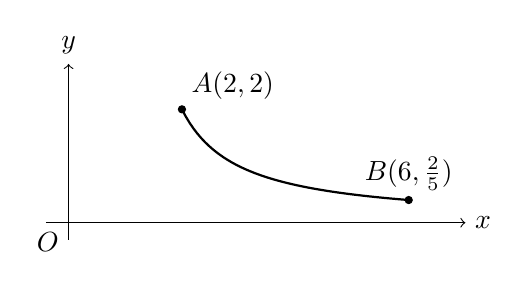
\begin{tikzpicture}[x=.72cm,y=.72cm]
\draw[->] (-.4,0)--(7,0) node[right]{$x$};\draw[->](0,-.3)--(0,2.8) node[above]{$y$};\node[below left] at (0,0){$O$};
\draw[thick,domain=2:6,samples=60] plot(\x,{2/(\x-1)});
\fill (2,2) circle(1.5pt) node[above right]{$A(2,2)$};\fill (6,.4) circle(1.5pt) node[above]{$B(6,\frac25)$};
\end{tikzpicture}
\q{14}函数 $y=[x]$ 的函数值表示不超过 $x$ 的最大整数，例如，$[-3.5]=-4$，$[2.1]=2$。已知函数 $f(x)=x|x-a|$，若函数 $y=[f(x)]$ 在区间 $(0,2)$ 上的值域为 $\{0,1\}$，则实数 $a$ 的取值范围是\blank。
\newpage
\textbf{四、解答题}（共5小题，共77分。解答应写出文字说明、证明过程或演算步骤。）
\q{15}（13分）设实数集 $\mathbb R$ 为全集，$A=\{x\mid y=\sqrt{x-2}\}$，$B=\{x\mid x^2-a<0\}$。
\subq{1}当 $a=4$ 时，求 $A\cup B$；
\subq{2}若 $A\cap B=\varnothing$，求实数 $a$ 的取值范围。
\par\vspace*{2.4cm}
\q{16}（15分）一家商店使用一架两臂不等长的天平称黄金，该天平左臂长为 $a$，右臂长为 $b$。一位顾客到店里想购买 $10\,\mathrm g$ 黄金。售货员先将 $5\,\mathrm g$ 的砝码放在天平左盘，取出一些黄金放在天平右盘中使天平平衡；再将 $5\,\mathrm g$ 的砝码放在天平右盘，再取出一些黄金放在天平左盘中使天平平衡；最后将两次称得的黄金一起交给顾客。（注：当天平平衡时，两侧的物体质量与对应力臂长的乘积相等。）
\subq{1}用含 $a,b$ 的式子表示两次称得的黄金克数之和 $M$；
\subq{2}试判断顾客拿到的黄金质量与 $10\,\mathrm g$ 的大小关系，并说明理由；
\subq{3}假设顾客得知自己拿到的黄金质量不超过 $12.5\,\mathrm g$，求该商店天平左臂与右臂长度之比 $\frac ab$ 的最大值。
\par\vspace*{2.4cm}
\q{17}（15分）给定函数 $f(x)=a^x$，$g(x)=\left(\frac1a\right)^x$（$0<a<1$）。$\forall x\in\mathbb R$，用 $m(x)$ 表示 $f(x),g(x)$ 中的最小者，记为 $m(x)=\min\{f(x),g(x)\}$。
\subq{1}求函数 $m(x)$ 的解析式；
\subq{2}已知函数 $F(x)=m(x)+b$ 的图象无限接近直线 $y=2$ 但又不与该直线相交，
\subq{i}请写出 $b$ 的值；
\subq{ii}解不等式 $F(k)>F(1-k)$。
\par\vspace*{2.4cm}
\newpage
\q{18}（17分）已知函数 $f(x)=x-\dfrac1{x-1}$。
\subq{1}判断并用定义证明函数 $f(x)$ 在 $(1,+\infty)$ 上的单调性；
\subq{2}函数 $y=f(x+a)-b$ 是奇函数，求 $a+b$ 的值；
\subq{3}若 $g(x)=a^x+1$（$a>1$），对 $\forall x_1\in(1,2]$，$\exists x_2\in(2,3]$，使得 $f(x_2)=g(x_1)$，求实数 $a$ 的取值范围。
\par\vspace*{6cm}
\q{19}（17分）已知幂函数 $f(x)=(m^2-m-1)x^{m^2-2m-1}$ 的图象关于 $y$ 轴对称，函数 $g(x)=f(x)-2(a+1)x+4a$。
\subq{1}求 $f(x)$ 的解析式；
\subq{2}若函数 $g(x)$ 在区间 $[0,3]$ 上的最小值为 $-1$，求 $a$；
\subq{3}若 $a>0$，函数 $h(x)=g(x)+2$，若对 $\forall t\in[1,2]$，$\exists x\in[t,t+1]$，使得 $h(h(x))<h(x)$，求实数 $a$ 的取值范围。
\par\vspace*{6cm}
\end{document}
